%%%%%%%%%%%%%%%%%%%%%%%%%%%%%%%%%%%%%%%%%%%%%%%%%%%%%%%%%%%%%%%%%%%%%%%%
% Plantilla TFG/TFM
% Escuela Politécnica Superior de la Universidad de Alicante
% Realizado por: Jose Manuel Requena Plens
% Contacto: info@jmrplens.com / Telegram:@jmrplens
%%%%%%%%%%%%%%%%%%%%%%%%%%%%%%%%%%%%%%%%%%%%%%%%%%%%%%%%%%%%%%%%%%%%%%%%

\chapter{Resultados}
\label{resultados}



  En esta sección se detallarán los resultados de los experimentos y se realizará un análisis comparativo entre ellos.


  En primer lugar....

\section{Algoritmo Genético}

  \textbf{NOTA} Ponemos aquí las figuras \ref{EvolucionHiperparametrosImage} y \ref{EvolucionF1ScoreImage} de evolución de hiperparámetros además de tabla de resultados \ref{BestGASolutionTable} en lugar de en metodologías?

  En la figura [\ref{EvolucionHiperparametrosImage}] se pueden visualizar la evolución de los parámetros del mejor individuo en cada generación.

  \begin{figure}[H]
      \centering
      \includesvg[scale=0.4]{archivos/5.Resultados/GA/EvolucionHiperparametros}
      \caption{Evolución de hiperparámetros a lo largo de las iteraciones.}
      \label{EvolucionHiperparametrosImage}
   \end{figure}

  \begin{figure}[H]
      \centering
      \includesvg[scale=0.4]{archivos/5.Resultados/GA/EvolucionF1Score}
      \caption{Evolución del macro F1 score a lo largo de las iteraciones.}
      \label{EvolucionF1ScoreImage}
   \end{figure}
   
  En la tabla \ref{BestGASolutionTable} se pueden observar el mejor individuo obtenido después de \textit{TODO: X} generaciones.

\section{XGBoost}

  \begin{figure}[H]
      \centering
      \includesvg[scale = 0.6]{archivos/5.Resultados/XGBoost/FeatureWeights}
      \caption{Pesos asignados por XGboost a las características.}
      \label{FeatureWeightsImage}
   \end{figure}

  \textbf{NOTA} Ponemos aquí las figuras de los pesos calculados \ref{FeatureWeightsImage} y la tabla de cáclulo de características \ref{PesosFinalesCaracteristicas}?

\section{Entrenamiento de modelos}

  
  \subsection{Gráficas de entrenamiento}

    Explicar las gráficas de evolución F1-score de las redes neuronales.


    \begin{figure}[h]
        \centering
        \includesvg[scale=0.3]{archivos/5.Resultados/CNN/1D/F1Score1D}
        \caption{Comparación de TODO(tipo) F1 score en validación y test CNN-1D.}
        \label{F1Score1DImage}
     \end{figure}


    \begin{figure}[h]
        \centering
        \includesvg[scale=0.3]{archivos/5.Resultados/CNN/2D/F1Score2D}
        \caption{Comparación de TODO(tipo) F1 score en validación y test CNN-2D.}
        \label{F1Score2DImage}
     \end{figure}


  \subsection{Reportes de clasificación}
       
    Explicar los reportes de clasificación con datos de \textbf{ENTRENAMIENTO.}

      \begin{table}[H]
        \centering
        \csvautotabular{archivos/5.Resultados/CNN/1D/1DCassificationReport.csv}
        \caption{Métricas CNN-1D.}
        \label{CNN1DMetrics}
      \end{table}

      \begin{table}[H]
        \centering
        \csvautotabular{archivos/5.Resultados/NB/NBCassificationReport.csv}
        \caption{Métricas Naive Bayes.}
        \label{NBMetrics}
      \end{table}

      \begin{table}[H]
        \centering
        \csvautotabular{archivos/5.Resultados/SVC/SVCCassificationReport.csv}
        \caption{Métricas SVC.}
        \label{SVCDMetrics}
      \end{table}

      \begin{table}[H]
        \centering
        \csvautotabular{archivos/5.Resultados/CNN/2D/2DCassificationReport.csv}
        \caption{Métricas CNN-2D.}
        \label{CNN2DMetrics}
      \end{table}


  \subsection{Matrices de confusión}

    Explicar las matrices de confusión con datos de \textbf{ENTRENAMIENTO.}

    \begin{figure}
        \centering
        \begin{subfigure}[b]{0.4\textwidth}
            \centering
            \includesvg[scale=0.4]{archivos/5.Resultados/CNN/1D/1DConfussionMatrix}
            \caption{Matriz de correlación CNN-1D.}
            \label{ConfussionMatrixImages:1D}
        \end{subfigure}
        % Añadir el espacio deseado, si se deja la linea en blanco la siguiente subfigura ira en una nueva linea
        \begin{subfigure}[b]{0.4\textwidth}
            \centering
            \includesvg[scale=0.4]{archivos/5.Resultados/CNN/2D/2DConfussionMatrix}
            \caption{Matriz de correlación CNN-2D.} 
            \label{ConfussionMatrixImages:2D}

        \end{subfigure}
        \begin{subfigure}[b]{0.4\textwidth}
            \centering
            \includesvg[scale=0.4]{archivos/5.Resultados/NB/NBConfussionMatrix}
            \caption{Matriz de correlación NB.}
            \label{ConfussionMatrixImages:NB}
        \end{subfigure}
        \begin{subfigure}[b]{0.4\textwidth}
            \centering
            \includesvg[scale=0.4]{archivos/5.Resultados/SVC/SVCConfussionMatrix}
            \caption{Matriz de correlación SVC.}
            \label{ConfussionMatrixImages:SVC}
        \end{subfigure}
        \caption{Matriz de correlación sobre el conjunto de test sobre los modelos aplicados.}
        \label{ConfussionMatrixImages}
     \end{figure}

  \subsection{Comparativa entre modelos}

    Explicar la comparativa de modelos con datos de \textbf{ENTRENAMIENTO.}


    \begin{figure}[h]
        \centering
        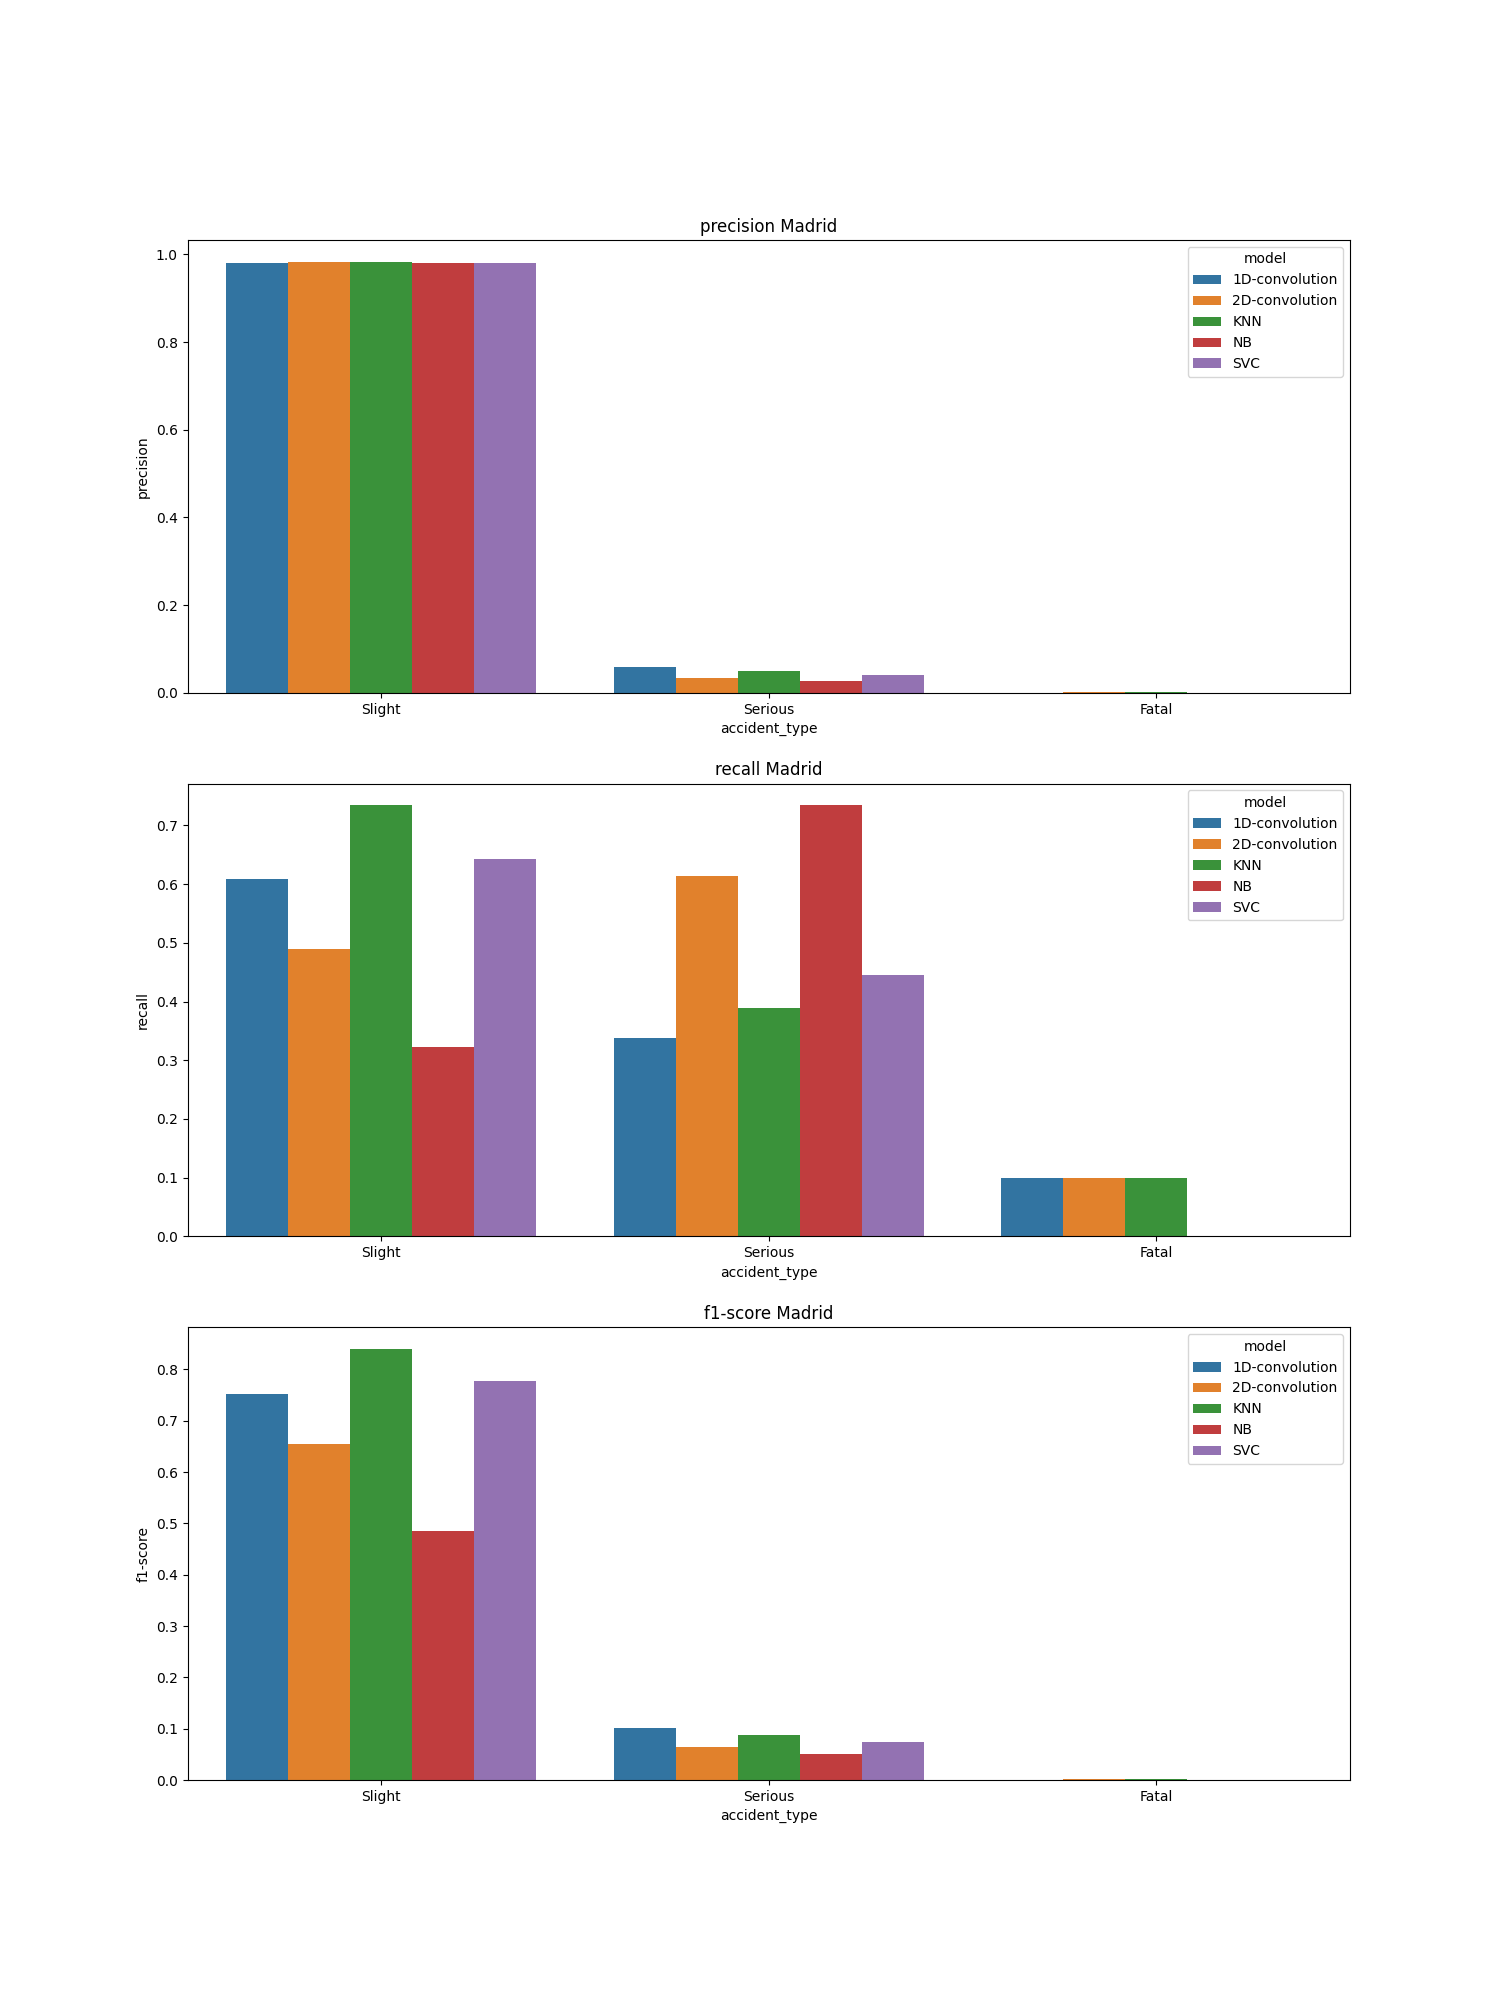
\includegraphics[width=10cm]{archivos/5.Resultados/Comparativa}
        \caption{Comparativa de las métricas predicciones de los modelos.}
        \label{ResultsImage}
     \end{figure}



\section{Predicciones de modelos}

  \subsection{Reportes de clasificación}

    Explicar los reportes de clasificación con datos de \textbf{TEST.}

    \begin{table}[H]
      \centering
      \csvautotabular{archivos/5.Resultados/CNN/1D/1DCassificationReport.csv}
      \caption{Métricas CNN-1D.}
      \label{CNN1DMetrics}
    \end{table}

    \begin{table}[H]
      \centering
      \csvautotabular{archivos/5.Resultados/NB/NBCassificationReport.csv}
      \caption{Métricas Naive Bayes.}
      \label{NBMetrics}
    \end{table}

    \begin{table}[H]
      \centering
      \csvautotabular{archivos/5.Resultados/SVC/SVCCassificationReport.csv}
      \caption{Métricas SVC.}
      \label{SVCDMetrics}
    \end{table}

    \begin{table}[H]
      \centering
      \csvautotabular{archivos/5.Resultados/CNN/2D/2DCassificationReport.csv}
      \caption{Métricas CNN-2D.}
      \label{CNN2DMetrics}
    \end{table}

  \subsection{Matrices de confusión}

    Explicar las matrices de confusión con datos de \textbf{TEST.}

    \begin{figure}
        \centering
        \begin{subfigure}[b]{0.4\textwidth}
            \centering
            \includesvg[scale=0.4]{archivos/5.Resultados/CNN/1D/1DConfussionMatrix}
            \caption{Matriz de confusión CNN-1D.}
            \label{ConfussionMatrixImages:1D}
        \end{subfigure}
        % Añadir el espacio deseado, si se deja la linea en blanco la siguiente subfigura ira en una nueva linea
        \begin{subfigure}[b]{0.4\textwidth}
            \centering
            \includesvg[scale=0.4]{archivos/5.Resultados/CNN/2D/2DConfussionMatrix}
            \caption{Matriz de confusión CNN-2D.} 
            \label{ConfussionMatrixImages:2D}

        \end{subfigure}
        \begin{subfigure}[b]{0.4\textwidth}
            \centering
            \includesvg[scale=0.4]{archivos/5.Resultados/NB/NBConfussionMatrix}
            \caption{Matriz de confusión NB.}
            \label{ConfussionMatrixImages:NB}
        \end{subfigure}
        \begin{subfigure}[b]{0.4\textwidth}
            \centering
            \includesvg[scale=0.4]{archivos/5.Resultados/SVC/SVCConfussionMatrix}
            \caption{Matriz de confusión SVC.}
            \label{ConfussionMatrixImages:SVC}
        \end{subfigure}

        \caption{Matrices de confusión de los modelos sobre el conjunto de entrenamiento.}
        \label{ConfussionMatrixImages}
     \end{figure}

  \subsection{Comparativa entre modelos}

    Explicar la comparativa de modelos con datos de \textbf{ENTRENAMIENTO.}


    \begin{figure}[h]
        \centering
        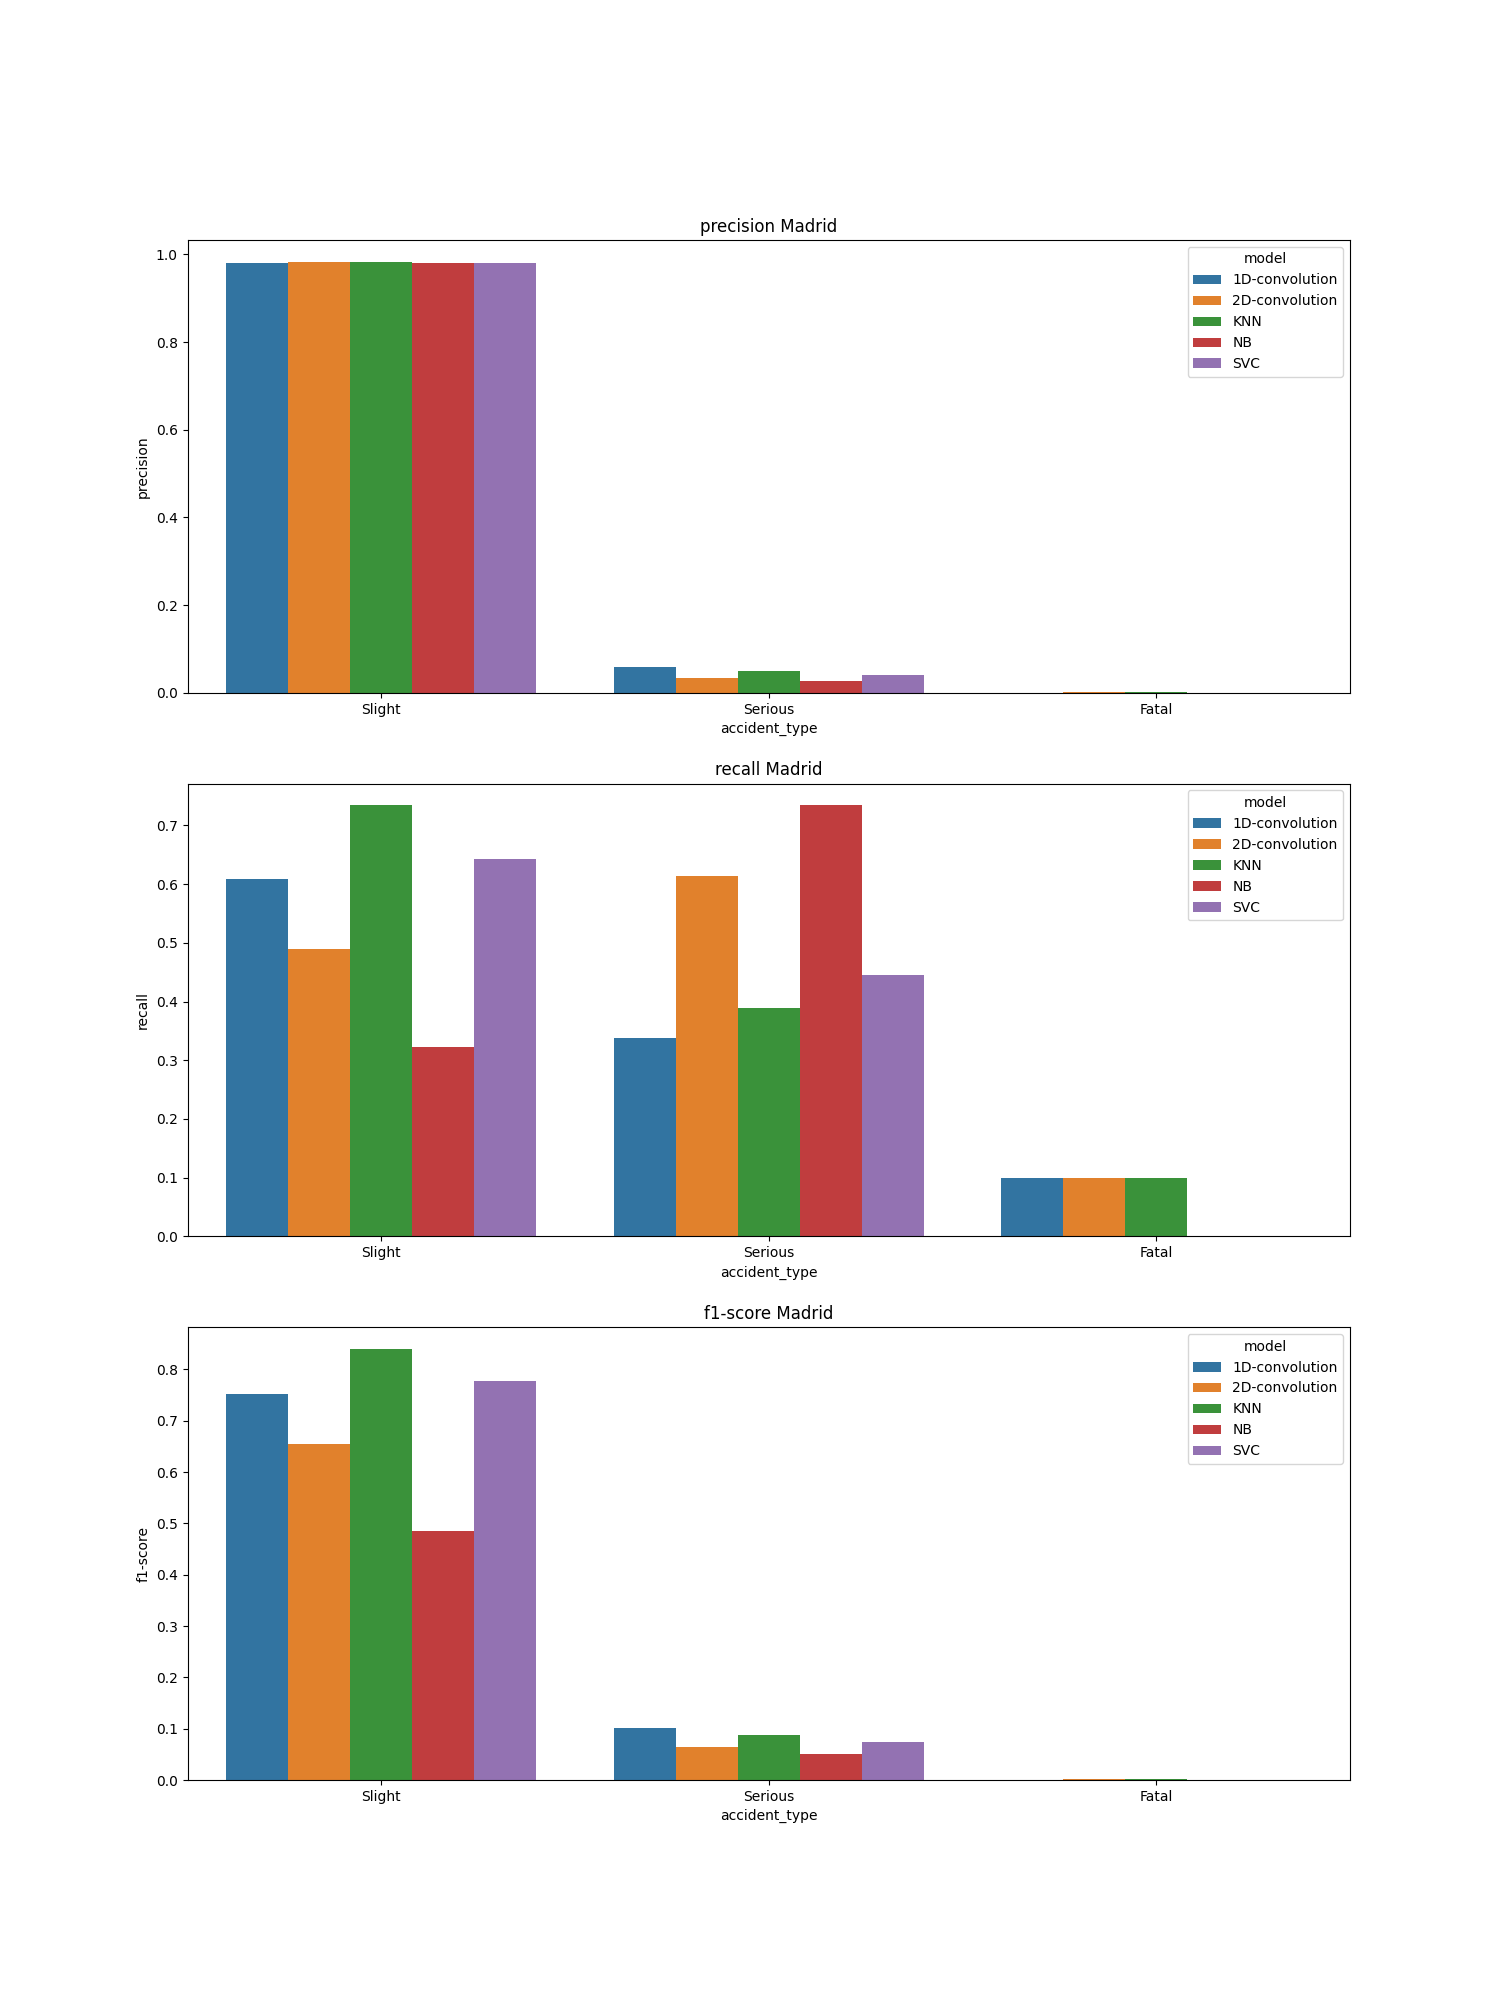
\includegraphics[width=10cm]{archivos/5.Resultados/Comparativa}
        \caption{Comparativa de las métricas predicciones de los modelos.}
        \label{ResultsImage}
     \end{figure}

